\documentclass[11pt, titlepage]{article}
\usepackage{amsmath,amsthm,amssymb}
\usepackage{hyperref, pgf, tikz}
\usepackage{fancyhdr}
\usetikzlibrary{arrows}
\usepackage[margin=1.25in]{geometry}
\usepackage{graphicx}                     
\pagestyle{fancy}
\usepackage{array}
%\usepackage{wrapfig}

\lhead{Lab \#03}
\rhead{\thepage}
\cfoot{}

\title{\Huge{The Addition and Resolution of Vectors: The Force Table} \\ \ \\ \huge Lab \#03}
\author{\Large{Alon Levin} \\ \emph{Lab Partners: Sophia Zheng, Avery Karlin}}
\date{\today}
\begin{document}

\maketitle

\begin{center}
\LARGE The Addtion and Resolution of Vectors: The Force Table
\end{center}

\section*{Objective}
The objectives of this lab are to learn two methods of adding sets of vectors (graphically and analytically) and thus to foster an appreciation of the differences between the two approaches.

\section*{Introduction}
A \textbf{vector} is a mathemaitcal concept which represents a quantity that has both a magnitude and a direction, unlike a \textbf{scalar} which has only a magnitude. Therefore, the process of adding vectors is more complex as well; there are three ways to find a vector sum: graphically, analytically, or experimentally.

\subsection*{Graphical Methods}
Vectors are represented graphically as arrows, with the length proportional to the magnitude and the direction represented by the direction the arrowhead points in. As can be seen in Fig. \ref{fig:1}, the graphical method can be approached in three ways.
\begin{figure}[!ht]
\centering
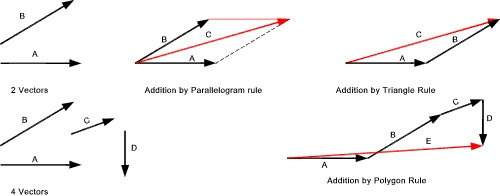
\includegraphics[scale=1, angle=0]{lab03_graphicvectors.jpg}
\caption{Three methods for graphical vector addition \label{fig:1}}
\end{figure} 
\begin{description}
	\item[Parallelogram] Given two vectors $\mathbf{A ~\text{and} ~B}$, a parallelogram could be constructed with $\mathbf{A} ~\text{and} ~\mathbf{B}$ as adjacent sides. The arrow diagonal of the parallelogram $\mathbf{R}$ is the resultant of $\mathbf{A} + \mathbf{B}$. In Fig. \ref{fig:1}, $\mathbf{R} ~\text{is denoted as} ~\mathbf{C}$.
	\item[Triangle] Given two vectors $\mathbf{A ~\text{and} ~B}$, the ``tail'' of $\mathbf{B}$ could be attached from the ``head'' of $\mathbf{A}$. The vector drawn from the tail of $\mathbf{A} ~\text{to the head of} ~\mathbf{B}$ is the resultant $\mathbf{R}$ of $\mathbf{A} + \mathbf{B}$. In Fig. \ref{fig:1}, $\mathbf{R} ~\text{is denoted as} ~\mathbf{C}$.
	\item[Polygon] For situations in which more than two vectors are added, the ``head-to-tail'' method employed in the \textbf{Triangle rule} can be employed repeatedly to form a polygon constructed of vectors. In Fig. \ref{fig:1}, $\mathbf{R} ~\text{is denoted as} ~\mathbf{E}$.
\end{description}

\subsection*{Analytical Methods}
The concept of a vector's magnitude and direction allow for more accurate mathematical methods of calculating vector sums.
\begin{figure}[!ht]
\centering
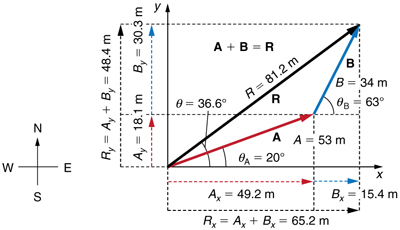
\includegraphics[scale=1.5, angle=0]{lab03_analyticalvectors.jpg}
\caption{Vector Sum broken into components and angles \label{fig:2}}
\end{figure} 

\noindent The components of a vector $\mathbf{V}$, with magnitude $V$ and angle $\theta$, are defined as
$$ V_x = V \cos\theta$$
\begin{equation} \label{eq:1}
V_y = V \sin\theta
\end{equation}
As shown by Fig. \ref{fig:2}, after vectors $\mathbf{A} ~\text{and} ~\mathbf{B}$ are placed head-to-tail, the values of their components and angles can be used in various ways to obtain the final values of the resultant $\mathbf{R}$'s magnitude and angle. To find the components, magnitude, and direction of $\mathbf{R}$, the following formulas are used:
$$R_x = A_x + B_x$$
$$R_y = A_y + B_y$$
$$R = \sqrt{R_x^2 + R_y^2}$$
\begin{equation} \label{eq:2}
\theta = \arctan({\frac{R_y}{R_x}})
\end{equation}

\subsection*{Experimental Methods}
A \textbf{force table} is essentially a circular table with a rim calibrated in degrees. Weight forces are applied to a central ring by means of systems of strings and pulleys, allowing for vectors to be modeled  both in direction (by varying the direction of the string) and in magnitude (by varying the weight pulling down on the string). The equlibirant $\mathbf{E}$ of several vectors can be found by creating an additional vector to balance out the pre-existing vectors. The equilibriant is a vector force of equal magnitude but opposite direction to the resultant; thus, by finding the equilibriant one can easily calculate the resultant $\mathbf{R} = -\mathbf{E}$
\section*{Procedure}

\pagebreak
\begin{figure}[!ht]
\centering
%\vspace*{1.5cm}
%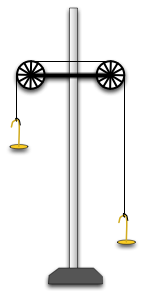
\includegraphics[scale=1.5, angle=0]{lab1.jpg}
\caption{Setup used for this experiment}
\end{figure}

\pagebreak
\section*{Data}
\begin{center}
%\begin{tabular}

%\end{tabular}
\begin{figure}[!ht]
\caption{caption}
\end{figure}
\end{center}

\pagebreak
\section*{Discussion}
\subsection*{Sample Calculations}

\subsection*{Analysis}

\section*{Conclusion}

\end{document}